\documentclass[11pt,french]{article} % police taille 11 car 10 c'est pour les terroristes
\usepackage{babel} % paquet qui permet de gérer les différentes langues
\usepackage{graphicx} % paquet pour inclure des images
\usepackage{float}
\usepackage{titling}
\usepackage{environ}
\usepackage{subfig}
\usepackage{listings}
\usepackage{xcolor}
\usepackage{amsmath,amsfonts,amssymb,amsthm}
\usepackage{geometry}
\geometry{legalpaper, margin=100pt}

\setlength{\parindent}{0pt}

\NewEnviron{NORMAL}{% environnement used to scale math equations 
    \scalebox{1.2}{$\BODY$} 
} 

\renewcommand{\contentsname}{Table des matières}


\definecolor{codegreen}{rgb}{0,0.6,0}
\definecolor{codegray}{rgb}{0.5,0.5,0.5}
\definecolor{codepurple}{rgb}{0.58,0,0.82}
\definecolor{backcolour}{rgb}{0.95,0.95,0.92}

\lstdefinestyle{mystyle}{
    backgroundcolor=\color{backcolour},   
    commentstyle=\color{codegreen},
    keywordstyle=\color{magenta},
    numberstyle=\tiny\color{codegray},
    stringstyle=\color{codepurple},
    basicstyle=\ttfamily\footnotesize,
    breakatwhitespace=false,         
    breaklines=true,                 
    captionpos=b,                    
    keepspaces=true,                 
    numbers=left,                    
    numbersep=5pt,                  
    showspaces=false,                
    showstringspaces=false,
    showtabs=false,                  
    tabsize=2
}
\lstset{style=mystyle}

% TODO : liens pour se deplacer vers section/figures
% TODO : ameliorer titres des figures
% TODO : revoir tout doc à la fin et faire des saut de ligne/pages pour rendre plus lisible
% TODO : ajouter critere Kalman

\begin{document}

\begin{figure}[t]
    \centering
		\advance\leftskip-0.2cm
    
\includegraphics[width=8cm]{inp_n7.png} % joli logo de l'N7
\end{figure}

\title{\vspace{0.5cm} \textbf{Rapport de bureau d'études\\Automatique Systèmes Cyber Physique}} 
\author{RAGOT Cyrian \\ Groupe K}
\renewcommand{\maketitlehookc}{%
	\vspace{3cm}
  \begin{center}
		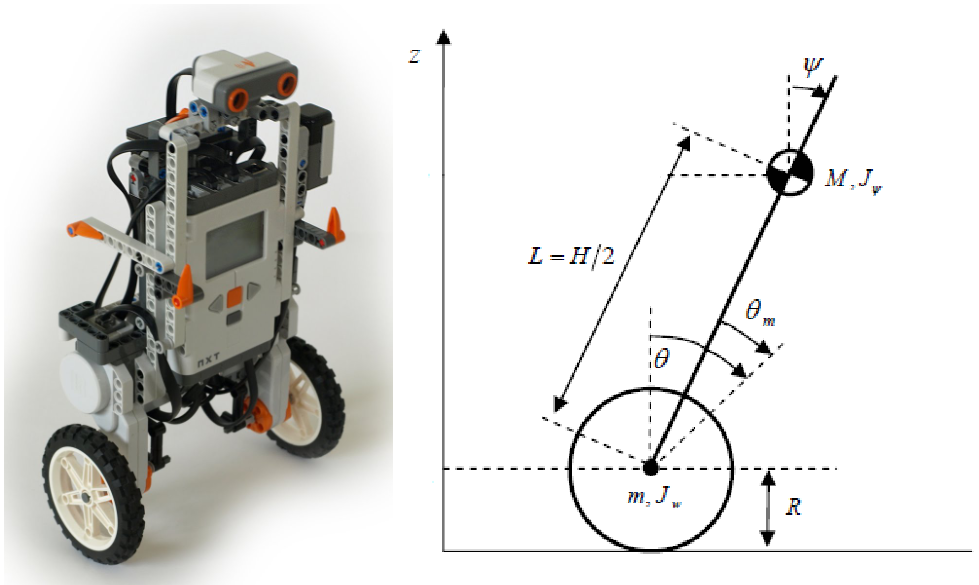
\includegraphics[width=14cm]{segway.png} % image segway 1ere page
  \end{center}
}
\date{\vspace{1cm}\vfill Département Sciences du Numérique - Première année \\
2023-2024 }

\maketitle

\newpage % génère un saut de page, en gros retour à la ligne mais pour une page
\tableofcontents % génère un sommaire des sections du document
\newpage

\section*{Introduction}
\addcontentsline{toc}{section}{\protect\numberline{}Introduction}

\quad Dans le cadre du cours d'automatique, nous nous sommes familiarisés avec les notions de système et des méthodes pour étudier la stabilité de ces systèmes selon certaines conditions. Nous avons aussi introduit des méthodes de contrôlabilité de ces systèmes. \\

\quad Nous avons pu alors appliquer ces connaissances dans un projet d'automatique qui s'est étendu sur plusieurs séances de TP. \\ \\ \\

\begin{large}
\textit{\textbf{\qquad Objectif : Stabiliser un robot Lego NXT verticalement. \\ \\ \\}}
\end{large}

\quad Pour remplir cet objectif, plusieurs modèles seront étudiés en passant de la théorie mathématique à des simulations de modèles créés sur Simulink et enfin de l'implémentation dans le robot. 



\newpage
\section{Modèle du pendule inversé}
\subsection{Contrôle par retour d'état}

\quad Dans cette partie, nous étudierons un modèle simple d'un pendule inversé contrôlé par retour d'état (figure \ref{fig:schema_pend_inv}) pour lequel on a accès aux variables de sortie. Le système contrôlé issu des équations physiques de la dynamique est \\


\begin{equation}
	\NORMAL{
  \left\{
    \begin{array}{l}
			\dot{x}_1(t) = x_2(t) \\
			\dot{x}_2(t) = \frac{g}{l}sin(x_1(t))-\frac{cos(x_1(t))u(t)}{l} \\
			\dot{x}_1(0) = x_{0,1} = \alpha_0 \\
			\dot{x}_2(0) = x_{0,2} = \dot\alpha_0, \\
    \end{array}
  \right.
	}
\end{equation}\\

\quad avec

\begin{description}
	\item[--] $\mathbf{g = 9.81 m/s^2}$ constante de gravité
	\item[--] $\mathbf{l = 10 m}$ longueur du pendule
	\item[--] $\mathbf{t_0 = 0 s}$ instant initial
	\item[--] $\boldsymbol{x(t) = (x_1(t), x_2(t))^\intercal = (\alpha(t), \dot\alpha(t))^\intercal}$ variable d'état 
	\item[--] $\boldsymbol{(x_e,u_e)^\intercal = (0,0,0)^\intercal}$ point de fonctionnement
	\item[--] $\boldsymbol{u(t)}$ contrôle par retour d'état
\end{description}

\begin{figure}[h]
    \centering
		\advance\leftskip-0.2cm
    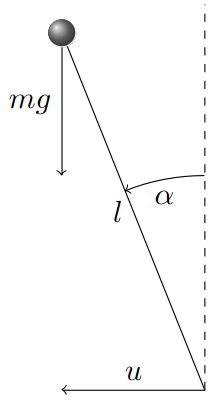
\includegraphics[width=3cm]{pendule_inverse.png}
		\caption{\textit{Schéma du pendule inversé}}
		\label{fig:schema_pend_inv}
\end{figure}
\vspace{0.5cm}

\subsubsection{Analyse du modèle théorique du pendule inverse}

\quad L'équation d'état est alors

\begin{equation}
	\NORMAL{
			\dot{x}(t) = f(x(t),u(t)), \\
	}
\end{equation}\\

\quad où 

\begin{equation}
	\NORMAL{
		f(x,u) = 
		\left(
		\begin{array}{c}
			x_2 \\
			\frac{g}{l}sin(x_1)-\frac{cos(x_1)u}{l} \\
    \end{array}
  \right)
	}
\end{equation}\\


\quad On souhaite stabiliser le système à l'origine (la position verticale du pendule inversé), cependant le système non contrôlé n'est pas stable à l'origine. En effet, lorsque $u = 0$, en passant par la jacobienne de $g$ au point de fonctionnement puis son polynôme caractéristique, on trouve la valeur propre $\sqrt{\frac{g}{l}}$ qui est à partie réelle strictement positive.\\

% TODO : on pourrait parler du critere de Kalman si ya de la place encore
% TODO : on pourrait mettre des equations pour le calcul de la vp aussi

\quad On choisit alors un contrôle en boucle fermée par retour d'état linéaire de la forme $u(t) = u_e + K(x(t) - x_e)$ avec $K = (k_1, k_2)$. Cherchons alors $K$ de manière à avoir un contrôle qui stabilise le système asymptotiquement en $x_e$.\\

\quad On boucle le système :\\

\begin{equation}
	\NORMAL{
			\dot{x}(t) = f(x(t),u_e + K(x(t)-x_e)) := g(x(t)) \\
	}
\end{equation}\\

\quad Alors $g(x_e) = f(x_e, u_e) = 0$ donc $x_e$ est un point d'équilibre de $\dot{x} = g(x)$. \\

\quad La matrice jacobienne associée est alors 

\begin{equation}
	\NORMAL{
		J_g(x) = 
		\left(
		\begin{array}{cc}
			0 & 1\\
			\frac{cos(x_1)}{l}(g-k_1)+\frac{u_e}{l}sin(x_1) & -\frac{cos(x_1)}{l}k_2 \\
    \end{array}
  \right)
	}
\end{equation}\\

\quad Au point de fonctionnement $(x_e,u_e) = (0,0,0)$ on a 

\begin{equation}
	\NORMAL{
		J_g(x_e) = 
		\left(
		\begin{array}{cc}
			0 & 1\\
			\frac{g-k_1}{l} & -\frac{k_2}{l} \\
    \end{array}
  \right)
	}
\end{equation}\\

\quad De plus, le contrôle stabilise asymptotiquement le système en $(x_e,u_e)$ si et seulement si les valeurs propres sont à parties réelles strictement négatives donc si et seulement si

\begin{equation}
	\NORMAL{
  \left\{
    \begin{array}{l}
			tr(J_g(x_e)) < 0 \\
			det(J_g(x_e)) > 0 \\
    \end{array}
  \right.
	}
\end{equation}\\

\quad Finalement,

\begin{equation} \label{eq:k12}
	\NORMAL{
  \left\{
    \begin{array}{l}
			k_1 > g \\
			k_2 > 0 \\
    \end{array}
  \right.
	}
\end{equation}\\

\subsubsection{Simulation du modèle sur Simulink} 

\quad Maintenant que l'on a compris comment le système contrôlé devrait réagir, nous allons effectuer des simulations sur Simulink où nous pourrons comparer le comportement du système pour différents cas d'étude. \\

\quad Les schémas blocs construits sur Simulink lors des séances de TP sont représentés sur les figures \ref{fig:simulink_controle_pend_inv}, \ref{fig:systeme_pend_inv} et \ref{fig:controle_pend_inv}. Nous étudierons les simulations avec les différents cas du tableau \ref{table:1}. On rappelle que $t_f$ est le temps de simulation en secondes. \\

\begin{figure}[H]
    \centering
    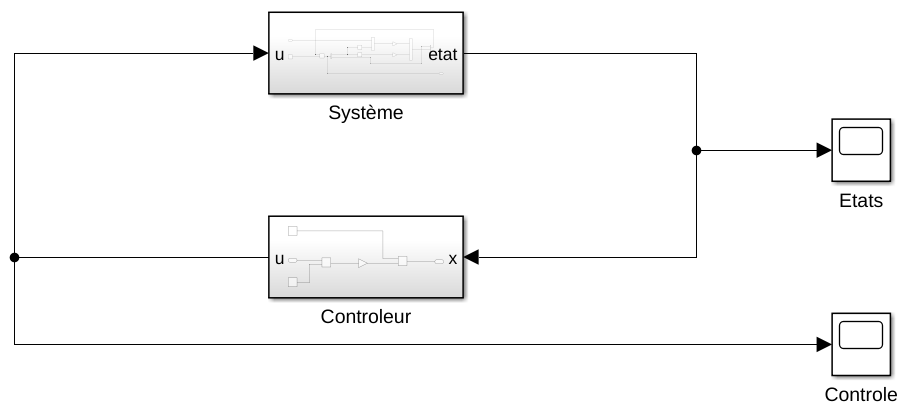
\includegraphics[width=9cm]{simulink_controle_pend_inv.png} 
		\caption{\textit{Schéma bloc du système contrôlé par retour d'état}}
		\label{fig:simulink_controle_pend_inv}
\end{figure}
\vspace{2cm}

\begin{figure}[H]
    \centering
		\advance\leftskip-2cm
    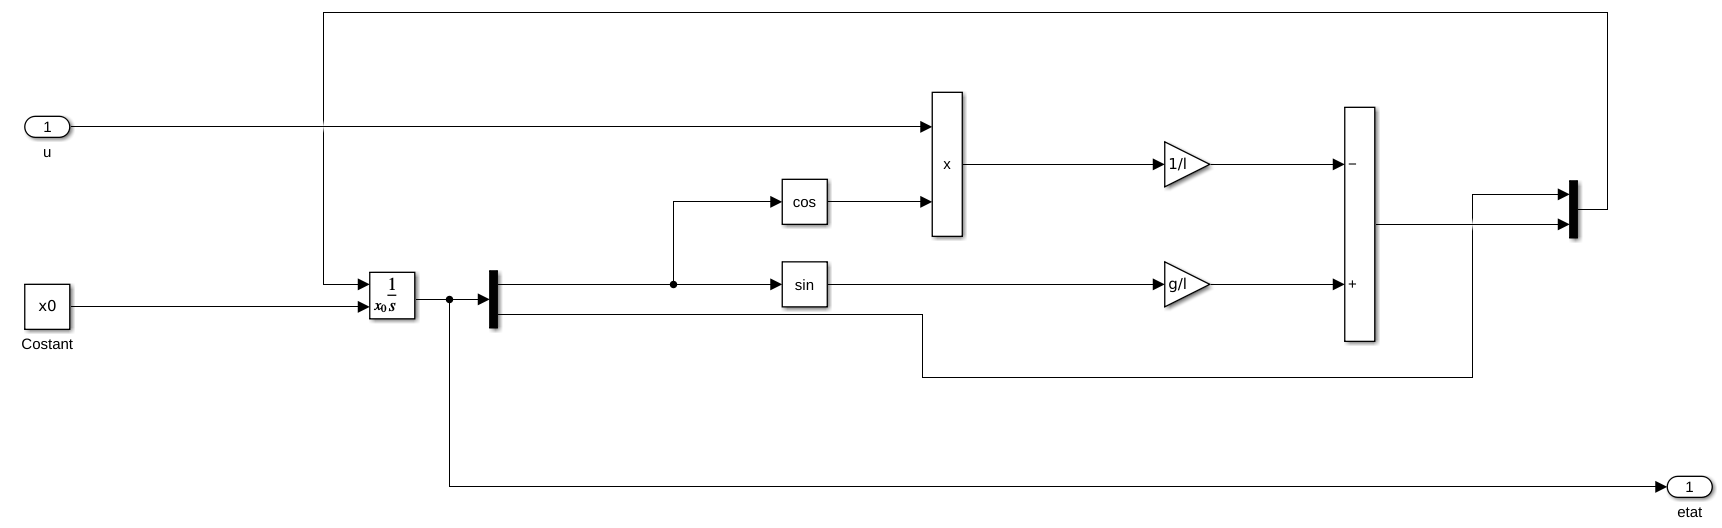
\includegraphics[width=19cm]{systeme_pend_inv.png} 
		\caption{\textit{Schéma bloc du système}}
		\label{fig:systeme_pend_inv}
\end{figure}
\vspace{0.5cm}

\begin{figure}[H]
    \centering
    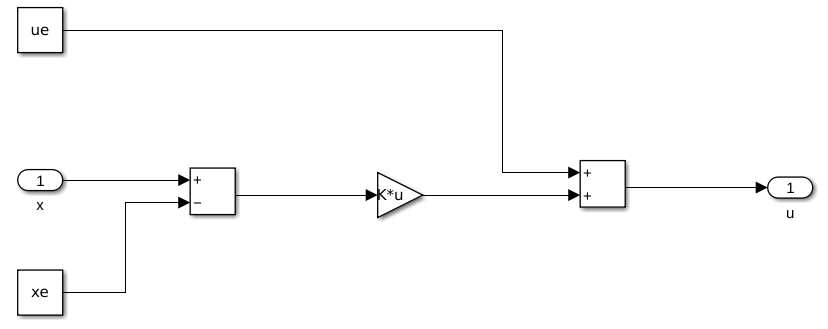
\includegraphics[width=11cm]{controle_pend_inv.png} 
		\caption{\textit{Schéma bloc du contrôleur}}
		\label{fig:controle_pend_inv}
\end{figure}
\vspace{0.5cm}

\begin{table}[h!]
\centering
\begin{tabular}{|c c c c c|} 
 \hline
 Cas & $x_0$ & $t_f$ & $K$ & Intégrateur \\ [0.5ex] 
 \hline\hline
 Cas 1 & $(\pi/20,0)$ & 10 & (30,10) & $ode45$ \\ 
 Cas 2 & $(\pi/20,0)$ & 100 & (10,1) & $ode45$ \\
 Cas 3 & $(\pi/20,0)$ & 100 & (10,1) & Euler, $ode1$ \\
 Cas 4 & $(\pi/20,0)$ & 1000 & (10,1) & Euler, $ode1$ \\
 Cas 5 & $(\pi/10,0)$ & 100 & (10,1) & $ode45$ \\ 
 Cas 6 & $(\pi/10,0)$ & 100 & (30,10) & $ode45$ \\ [1ex] 
 \hline
\end{tabular}
\caption{\textit{Données pour différents cas d'étude du contrôle par retour d'état}}
\label{table:1}
\end{table} 

\quad Commentons les résultats des simulations obtenues pour ces cas d'étude. \\

\quad Prenons les deux premiers cas dont les courbes sont représentées en figure \ref{fig:cas_1_2}. Les conditions pour la stabilisation sont vraies aux alentours du point de fonctionnement, or la valeur de $x_0$ est bien proche de $x_e=(0,0)$. De plus, les conditions de l'équation (\ref{eq:k12}) sont vérifiées dans ces deux cas. On a bien un système qui est stabilisé. Pour le cas 2, on diminue le gain $K$ du contrôle, ceci prolonge le temps de réponse du système puisque le contrôle a moins d'impact. \\

\begin{figure}[H]%
    \centering
		\noindent\makebox[\textwidth]{
		\subfloat[\centering{Cas 1}]{{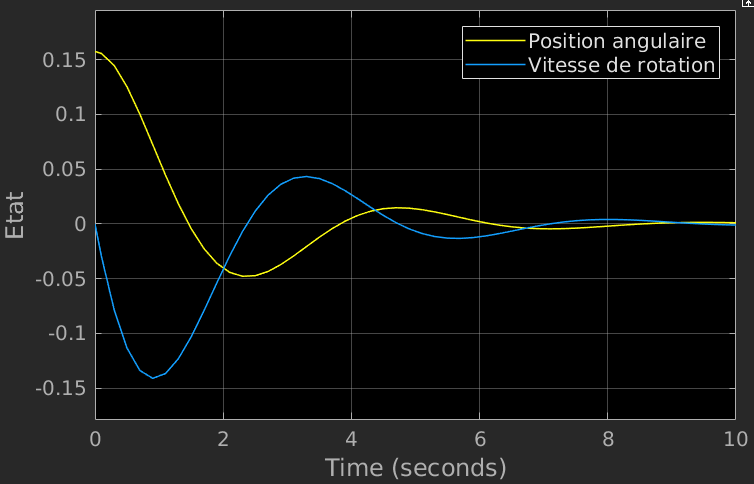
\includegraphics[width=9cm]{tp2_cas_11.png}}}%
		\qquad
		\subfloat[\centering{Cas 2}]{{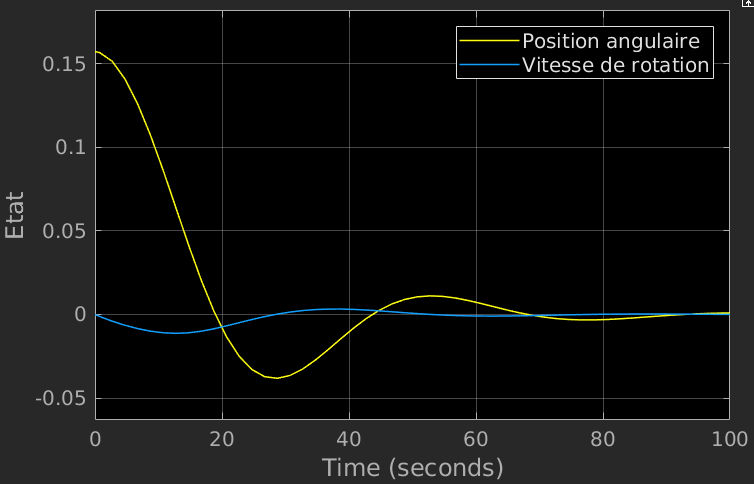
\includegraphics[width=9cm]{tp2_cas_12.png}}}}%
		\caption{\textit{Comparaison du changement de gain}}%
		\label{fig:cas_1_2}%
\end{figure}
\vspace{0.5cm}

\quad Ensuite, pour les cas 3 et 4 (figure \ref{fig:cas_3_4}), on change d'algorithme d'intégration. Le cas 3 montre une perte de précision, les oscillations sont plus larges qu'au cas 2, mais restent stabilisées. En revanche, pour le cas 4, on augmente seulement le temps de simulation et la courbe de l'état devient absurde. En effet, l'intégrateur de l'algorithme d'Euler $ode1$ utilise un pas qui dépend de la durée de simulation. Ici, le pas est trop grand et provoque une simulation incorrecte. \\

\begin{figure}[H]%
    \centering
		\noindent\makebox[\textwidth]{
		\subfloat[\centering{Cas 3}]{{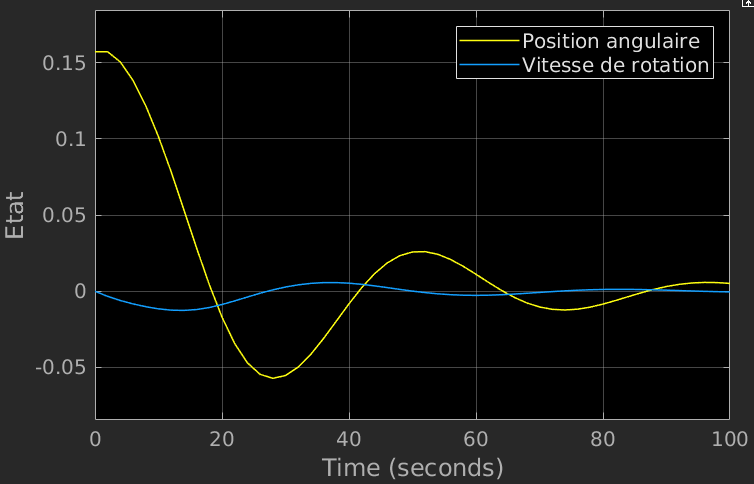
\includegraphics[width=9cm]{tp2_cas_13.png}}}%
		\qquad
		\subfloat[\centering{Cas 4}]{{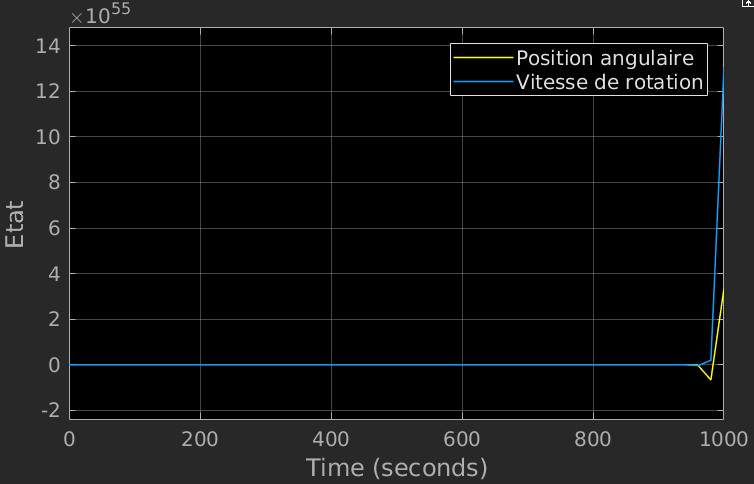
\includegraphics[width=9cm]{tp2_cas_14.png}}}}%
		\caption{\textit{Comparaison du changement d'intégrateur}}%
		\label{fig:cas_3_4}%
\end{figure}
\vspace{0.5cm}

\quad Enfin, on repasse sur le premier intégrateur. Les cas 5 et 6 (figure \ref{fig:cas_5_6}) ont été obtenus en modifiant l'état initial $x_0$ que l'on a pris plus loin du point de fonctionnement, on a choisi un angle initial plus grand $\pi/10$ au lieu de $\pi/20$. En gardant un gain faible $K$, on ne stabilise plus le système, l'état diverge au cas 5. Cependant, si on augmente à nouveau $K$ à la valeur du cas 1, on peut re-stabiliser le système (cas 6) puisqu'on donne plus d'importance au contrôle. \\

\begin{figure}[H]%
    \centering
		\noindent\makebox[\textwidth]{
		\subfloat[\centering{Cas 5}]{{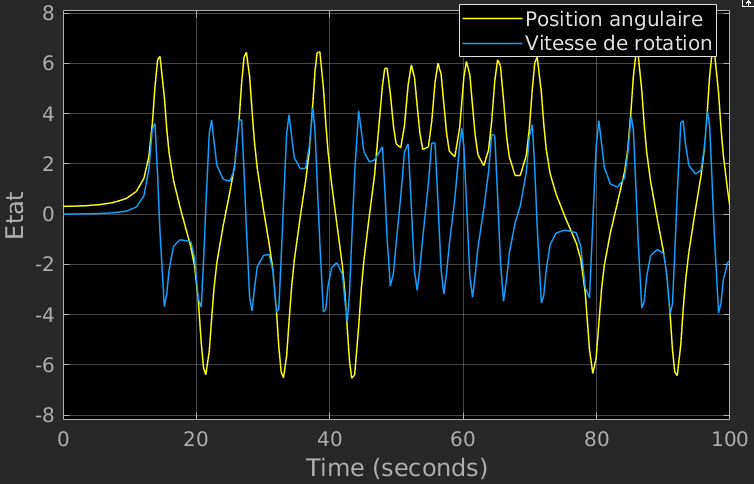
\includegraphics[width=9cm]{tp2_cas_15.png}}}%
		\qquad
		\subfloat[\centering{Cas 6}]{{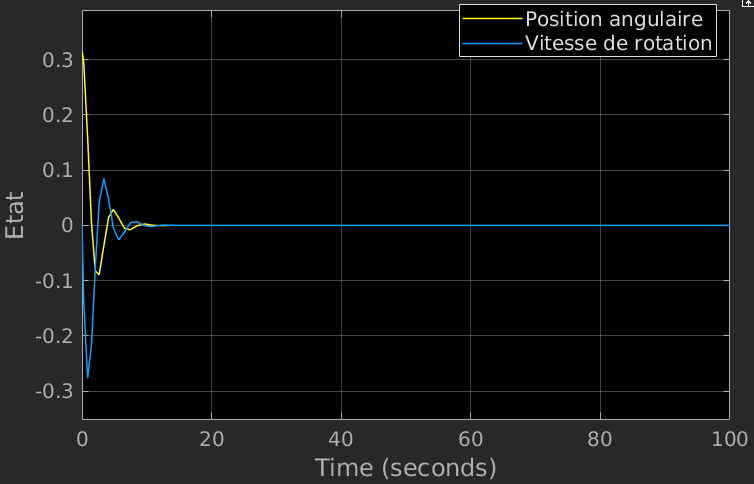
\includegraphics[width=9cm]{tp2_cas_16.png}}}}%
		\caption{\textit{Comparaison du changement d'état initial}}%
		\label{fig:cas_5_6}%
\end{figure}
\vspace{0.5cm}




\subsection{Contrôle par retour de sortie avec capteur}

\quad Nous avons pu contrôler correctement le système à l'aide des variables de sorties de position angulaire et de vitesse, cependant, sur un système réel, on a pas toujours accès à toutes les variables de sorties. On va donc maintenant supposer que l'on a accès qu'à la valeur $\dot\alpha$ à l'aide d'un capteur sur le système. Il faut alors reconstruire $\alpha$ à l'aide d'un prédicteur. Pour cela, on utilise un intégrateur continu. \\

\quad Le schéma bloc réalisé sur Simulink en séance de TP reste le même pour le bloc du système simple (figure \ref{fig:systeme_pend_inv}) et le bloc du contrôleur (figure \ref{fig:controle_pend_inv}), on ajoute simplement le capteur et le prédicteur sur la figure \ref{fig:simulink_capteur_pend_inv}. Les blocs du prédicteur et du capteur sont représentés respectivement sur les figures \ref{fig:predicteur_pend_inv} et \ref{fig:capteur_pend_inv}. Nous étudierons les simulations avec les différents cas du tableau \ref{table:2}. \\

\begin{figure}[H]
    \centering
    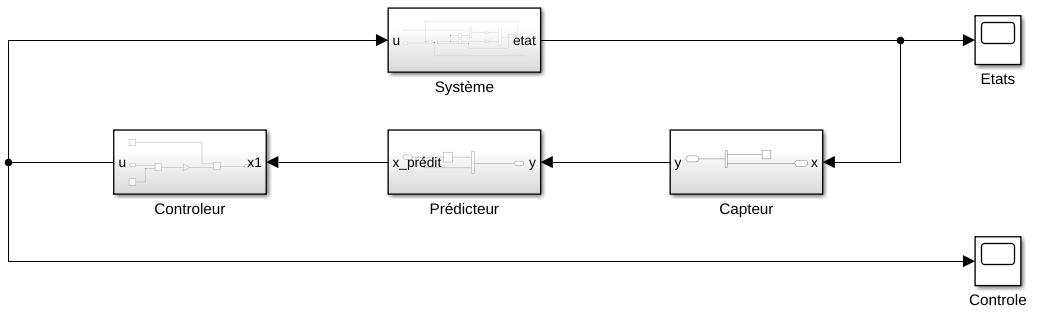
\includegraphics[width=12cm]{simulink_capteur_pend_inv.png} 
		\caption{\textit{Schéma bloc du système contrôlé par retour de sortie}}
		\label{fig:simulink_capteur_pend_inv}
\end{figure}
\vspace{0.5cm}

\begin{figure}[H]
    \centering
    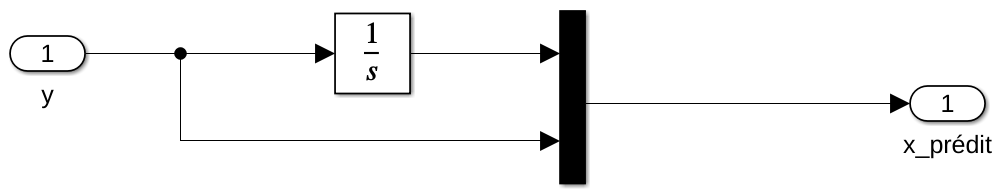
\includegraphics[width=11cm]{predicteur_pend_inv.png} 
		\caption{\textit{Schéma bloc du prédicteur}}
		\label{fig:predicteur_pend_inv}
\end{figure}
\vspace{0.5cm}

\begin{figure}[H]
    \centering
    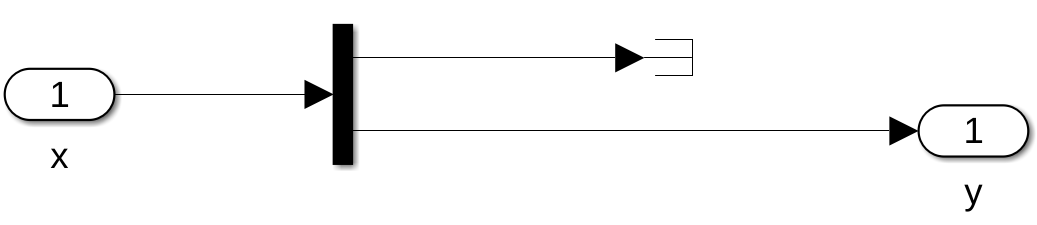
\includegraphics[width=11cm]{capteur_pend_inv.png} 
		\caption{\textit{Schéma bloc du capteur}}
		\label{fig:capteur_pend_inv}
\end{figure}
\vspace{0.5cm}

\begin{table}[h!]
\centering
\begin{tabular}{|c c c c c c|} 
 \hline
 Cas & $x_0$ & $t_f$ & $K$ & Pas & Intégrateur \\ [0.5ex] 
 \hline\hline
 Cas 1 & $(\pi/20,0)$ & 100 & (10,1) & par défaut & $ode45$ \\ 
 Cas 2 & $(\pi/20,0)$ & 100 & (10,1) & 0.001 & Euler, $ode1$ \\
 Cas 3 & $(\pi/20,0)$ & 100 & (10,1) & 5 & Euler, $ode1$ \\ [1ex]
 \hline
\end{tabular}
\caption{\textit{Données pour différents cas d'étude du contrôle par retour de sortie}}
\label{table:2}
\end{table}

\quad Nous pouvons observer sur les trois courbes (figure \ref{fig:courbes_capteurs}) des points indiquant le pas de l'intégrateur choisi. \\

\quad Pour le premier cas, nous avons utilisé l'intégrateur plus performant $ode45$ qui ne nécessite pas de préciser le pas qui est fixé par défaut. De plus, la courbe est similaire à celle du cas 2 de la figure \ref{fig:cas_1_2}, notre contrôle donc fonctionne aussi bien lorsque le signal est reconstitué au travers d'un capteur pour cet intégrateur. \\

\quad Le second cas utilise l'intégrateur d'Euler, $ode1$ avec un pas fixé à $0.001$ contrairement à la figure \ref{fig:cas_3_4} où le pas était automatique. Ici, le pas choisi est suffisamment petit pour avoir un modèle correct qui donne un résultat similaire au cas 1. Cependant, le premier intégrateur est très certainement moins lourd et plus rapide que celui-ci vu le nombre de points calculé au cas 2. \\

\quad Quant au dernier cas, on a pris un pas de $5$ bien trop grand pour l'intégrateur d'Euler $ode1$ ce qui entraîne une mauvaise simulation avec un temps de réponse plus grand mais on a toujours une stabilisation.

\begin{figure}[H]%
	\centering
	\noindent\makebox[\textwidth]{
		\subfloat[Cas 1]{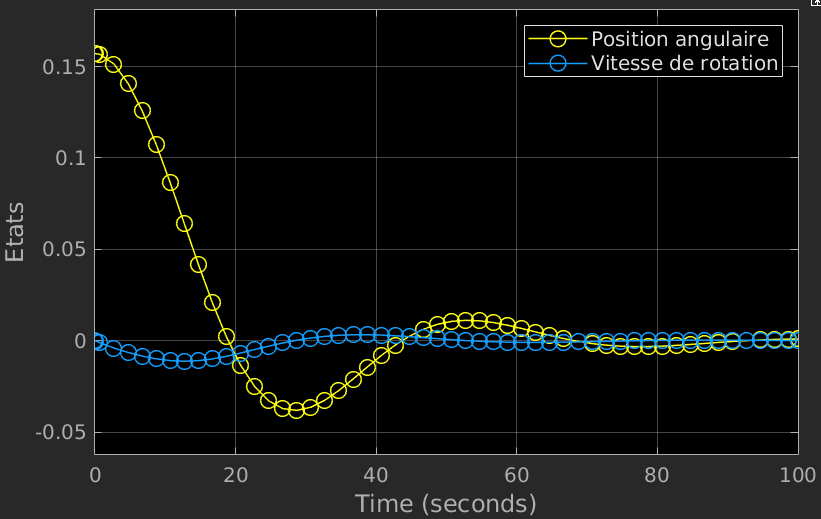
\includegraphics[width=9cm]{tp2_cas_21.png}} \qquad
		\subfloat[Cas 2]{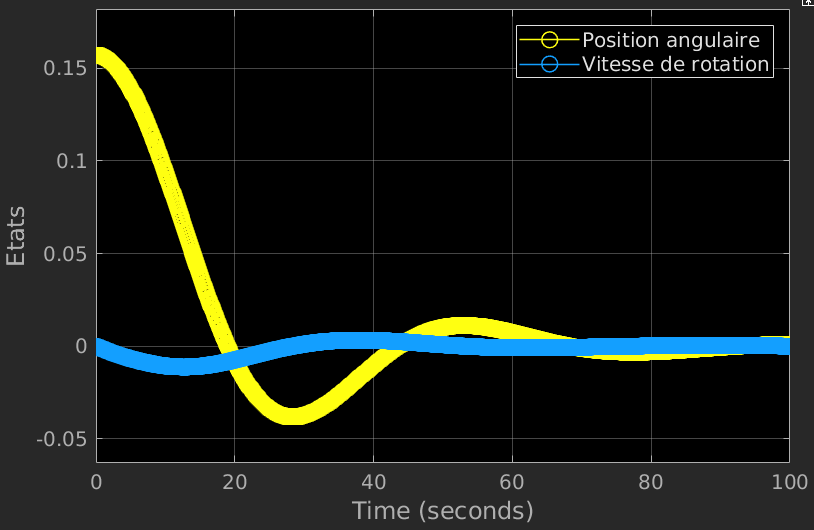
\includegraphics[width=9cm]{tp2_cas_22.png}}} \\
		\subfloat[Cas 3]{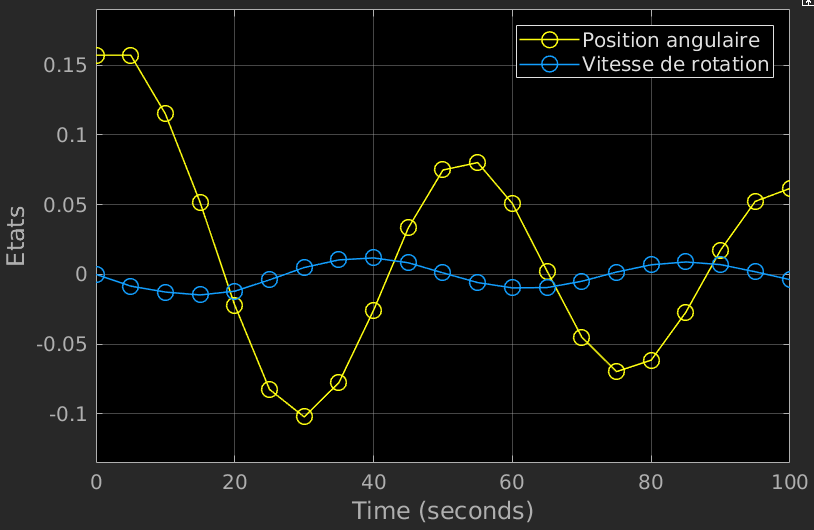
\includegraphics[width=9cm]{tp2_cas_23.png}}
		\caption{\textit{Comparaison de l'algorithme d'intégration utilisé}}
		\label{fig:courbes_capteurs}%
\end{figure}
\vspace{0.5cm}


\newpage
\section{Modèle du robot Lego}

\quad Après avoir étudié un modèle simple de pendule inverse, tentons de modéliser le système plus compelxe du robot Lego NXT qui s'appuie sur celui du pendule inverse. \\

\subsection{Contrôle par retour d'état}

\quad Nous allons à nouveau étudier le modèle avec contrôle par retour d'état. Cette fois les équations de la dynamique sont plus complexes car elles font intervenir l'inertie du robot et deux autres variables d'état supplémentaires : la position angulaire des roues $\theta$ et leur vitesse angulaire $\dot\theta$. On a donc $x(t) = (x_1(t),x_2(t),x_3(t),x_4(t))^\intercal = (\theta(t),\alpha(t),\dot\theta(t),\dot\alpha(t))^\intercal$ et $x_e = (0,0,0,0)^\intercal$. \\

\subsubsection{Analyse du modèle théorique du robot}

\quad L'équation d'état reste la même que dans 1.1.1 (voir (2)) mais $f$ est définie différemment. Nous n'irons par dans les détails pour rester dans le cadre de notre étude.\\
Comme pour la partie 1.1.1, on boucle le système avec le contrôle $u(t)$ (voir (4)) et $K \in \mathbb{R}$. Puis, on trouve la matrice jacobienne au point de fonctionnement sous la forme

\begin{equation}
	\NORMAL{
			J_g(x_e) = A + BK \\
	}
\end{equation}\\

où $A \in \mathbb{M}_4$ et $B \in \mathbb{R}^4$. \\

\quad Finalement, la stabilisation du système va dépendre des valeurs propres de $J_g(x_e)$, on aimerait alors trouver $K$ tel que ces valeurs propres soient strictement négatives. On prendra les valeurs propres contenues dans $V = (-136.5905, -2.6555, -3.5026, -5.9946)$. \\

\subsubsection{Simulation du modèle sur Simulink}

\quad Nous pouvons maintenant effectuer des simulations du robot Lego sur Simulink. La figure \ref{fig:simulink_tp3_1} représente le schéma bloc du système contrôlé par retour d'état, le bloc de contrôle étant le même que celui de la figure \ref{fig:controle_pend_inv}. La table \ref{table:3} référencie les différents cas étudiés lors des simulations. \\

\quad Les équations de la dynamique sont ici décrites par une fonction matlab fournie pour simuler le système. De plus, on trouve $K$ en calculant les matrices A et B puis en utilisant la fonction $place(A,B,V)$ qui retourne $-K$ dans un fichier matlab à part. L'algorithme d'intégration utilisé est $ode45$. \\

\begin{figure}[H]
    \centering
    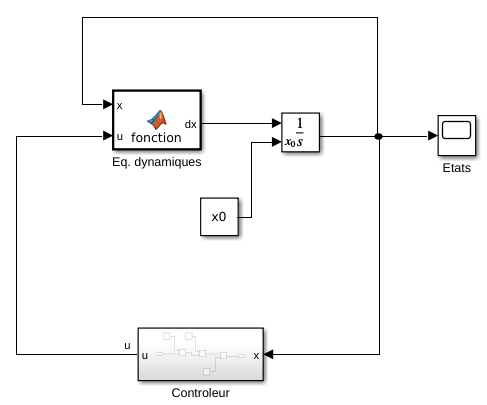
\includegraphics[width=8cm]{simulink_tp3_1.png} 
		\caption{\textit{Schéma bloc du système contrôlé du robot Lego}}
		\label{fig:simulink_tp3_1}
\end{figure}
\vspace{0.5cm}

\begin{table}[h!]
\centering
\begin{tabular}{|c c c|} 
 \hline
 Cas & $x_0$ & $t_f$ \\ [0.5ex] 
 \hline\hline
 Cas 1 & $(0,0,0,0)$ & 2 \\ 
 Cas 2 & $(0,\pi/5,0,0)$ & 5 \\ 
 Cas 3 & $(0,\pi/10,0,0)$ & 5 \\ [1ex] 
 \hline
\end{tabular}
\caption{\textit{Données pour différents cas d'étude du contrôle par retour d'état}}
\label{table:3}
\end{table}

\quad Les résultats sont représentés sur la figure \ref{fig:robot_controle}. On remarque pour le cas 1 que l'état reste constant nul pour un état initial nul, le système ne dégénère donc pas au point de fonctionnement. Pour des états initiaux non nuls (cas 2 et 3), on visualise bien une stabilisation du système contrôlé. Enfin, on remarque que pour une position angulaire initiale plus faible (cas 3), les oscillations sont moins fortes, ce qui est normal puisque le système démarre plus proche du point de fonctionnement. \\ 

\begin{figure}[H]%
	\centering
	\noindent\makebox[\textwidth]{
		\subfloat[Cas 1]{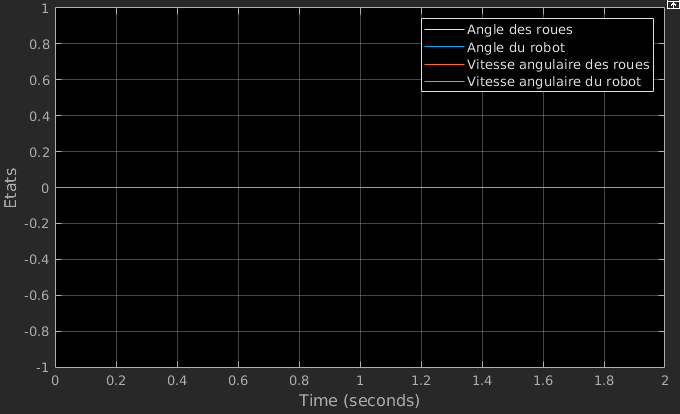
\includegraphics[width=9cm]{tp3_cas_11.png}} \qquad
		\subfloat[Cas 2]{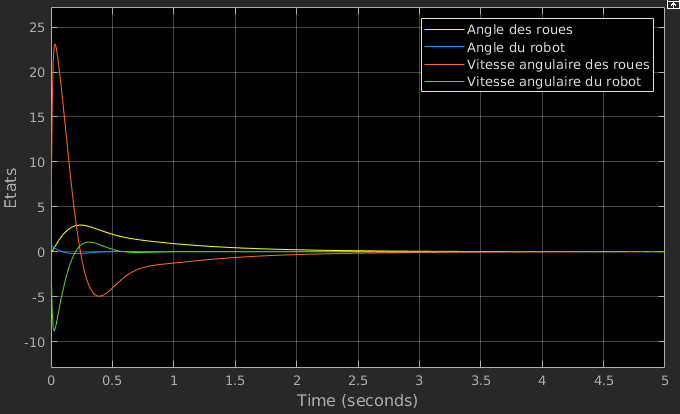
\includegraphics[width=9cm]{tp3_cas_12.png}}} \\
		\subfloat[Cas 3]{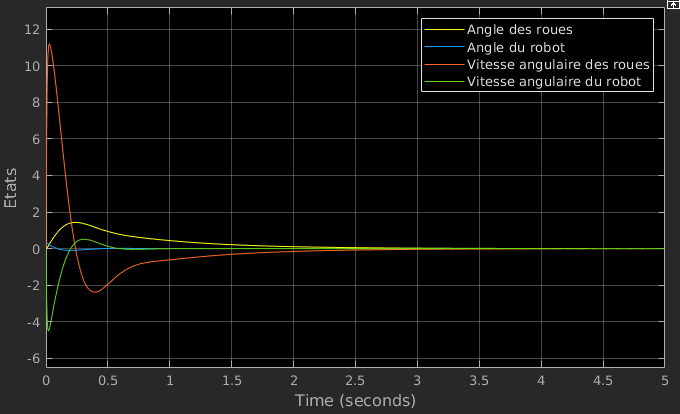
\includegraphics[width=9cm]{tp3_cas_13.png}}
		\captionsetup{justification=centering}
		\caption{\textit{Résultats du contrôle par retour d'état du robot Lego pour différents états initiaux}}
		\label{fig:robot_controle}%
\end{figure}
\vspace{0.5cm}


\subsection{Contrôle par retour de sortie avec capteur}

\quad Dans cette partie nous allons encore une fois effectuer un contrôle par retour de sortie en considérant que l'on a accès qu'aux valeurs de la vitesse angulaire $\dot\alpha = x_4$ du robot et de la position angulaire des roues $\theta = x_1$ à l'aide de capteurs. Encore une fois nous avons besoin d'un prédicteur pour reconstruire l'information des deux autres composantes manquantes. \\

\quad Le schéma bloc réalisé en figure \ref{fig:simulink_tp3_2_systeme} est similaire à celui de la figure \ref{fig:simulink_tp3_1} mais on y ajoute un bloc pour le capteur (figure \ref{fig:simulink_tp3_2_capteur}) et pour le prédicteur (figure \ref{fig:simulink_tp3_2_predicteur}). \\

\begin{figure}[H]
    \centering
    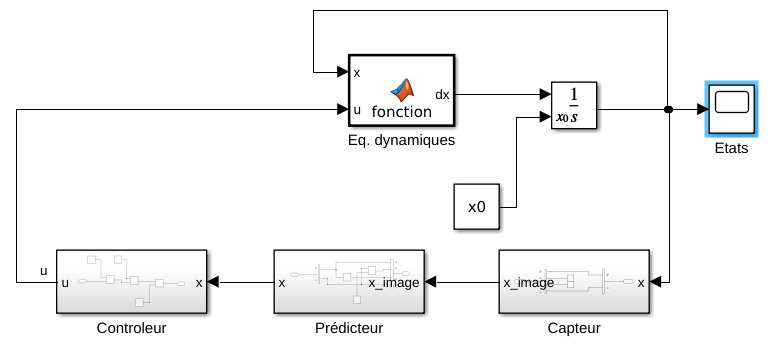
\includegraphics[width=12cm]{simulink_tp3_2_systeme.png} 
		\caption{\textit{Schéma bloc du système contrôlé par retour de sortie du robot Lego}}
		\label{fig:simulink_tp3_2_systeme}
\end{figure}
\vspace{0.5cm}

\begin{figure}[H]
    \centering
    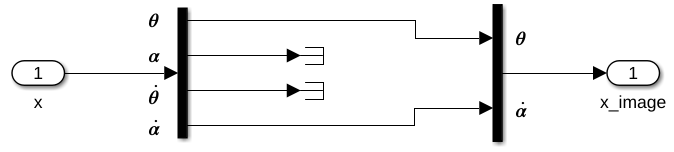
\includegraphics[width=12cm]{simulink_tp3_2_capteur.png} 
		\caption{\textit{Schéma bloc du capteur}}
		\label{fig:simulink_tp3_2_capteur}
\end{figure}
\vspace{0.5cm}

\begin{figure}[H]
    \centering
    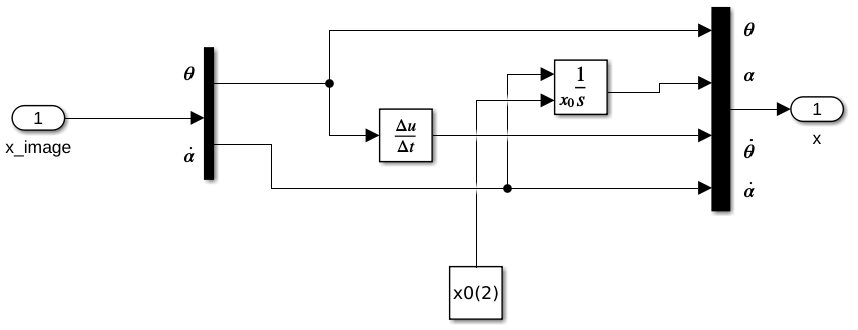
\includegraphics[width=12cm]{simulink_tp3_2_predicteur.png} 
		\caption{\textit{Schéma bloc du prédicteur}}
		\label{fig:simulink_tp3_2_predicteur}
\end{figure}
\vspace{0.5cm}

\quad Pour la simulation, on étudie les mêmes cas que dans la partie 2.1.2 qui sont donnés en table \ref{table:3}. Les résultats sont donnés en figure \ref{fig:robot_capteur}. Les courbes obtenues semblent être les mêmes que celles de la figure \ref{fig:robot_controle} pour le contrôle par retour d'état, ce qui est normal en utilisant l'intégrateur performant $ode45$. Les conclusions sont donc les mêmes. Avec un bon intégrateur, on peut toujours stabiliser aussi bien le système avec ou sans capteur. \\

\begin{figure}[H]%
	\centering
	\noindent\makebox[\textwidth]{
		\subfloat[Cas 1]{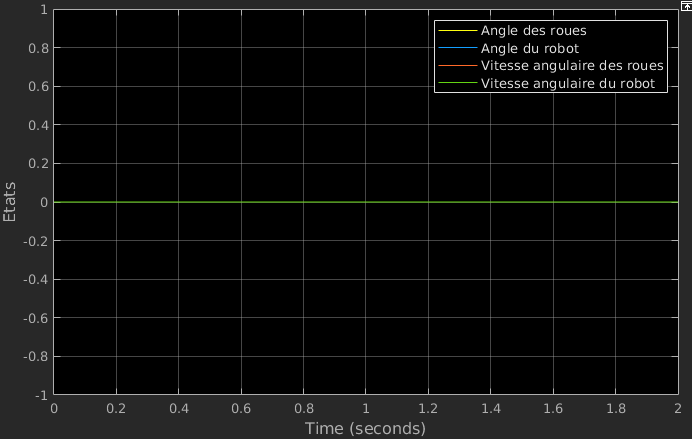
\includegraphics[width=9cm]{tp3_cas_21.png}} \qquad
		\subfloat[Cas 2]{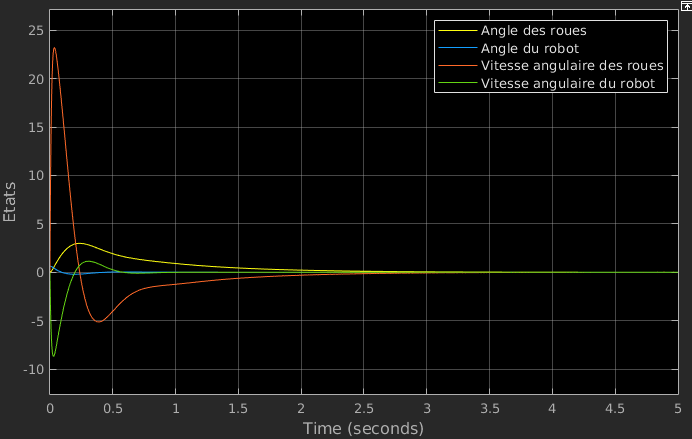
\includegraphics[width=9cm]{tp3_cas_22.png}}} \\
		\subfloat[Cas 3]{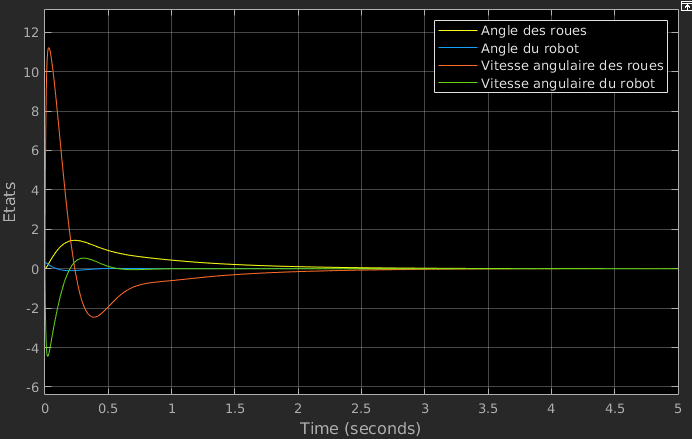
\includegraphics[width=9cm]{tp3_cas_23.png}}
		\captionsetup{justification=centering}
		\caption{\textit{Résultats du contrôle par retour de sortie du robot Lego pour différents états initiaux}}
		\label{fig:robot_capteur}%
\end{figure}
\vspace{0.5cm}


\subsection{Modèle hybride par discrétisation}

\quad Enfin, il reste un aspect que l'on n'a pas traité pour le pendule inverse et qui est important pour un système réel, c'est la prise en compte de signaux discrets. En effet, le logiciel implanté dans le robot, qui calcul le contrôle et la prédiction, fonctionne avec un signal discret tandis que le système représentant la physique est continu. On change donc les blocs du capteur et du prédicteur sur Simulink pour simuler un signal discret (voir figures \ref{fig:simulink_tp3_3_capteur} et \ref{fig:simulink_tp3_3_predicteur}). Le reste du système reste le même que précédemment (figure \ref{fig:simulink_tp3_2_systeme}). \\

\begin{figure}[H]
    \centering
    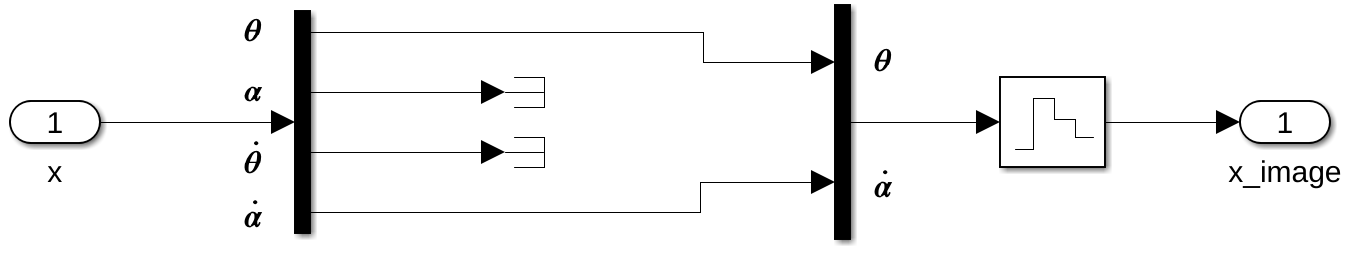
\includegraphics[width=12cm]{simulink_tp3_3_capteur.png} 
		\caption{\textit{Schéma bloc du capteur avec signal discret}}
		\label{fig:simulink_tp3_3_capteur}
\end{figure}
\vspace{0.5cm}

\begin{figure}[H]
    \centering
    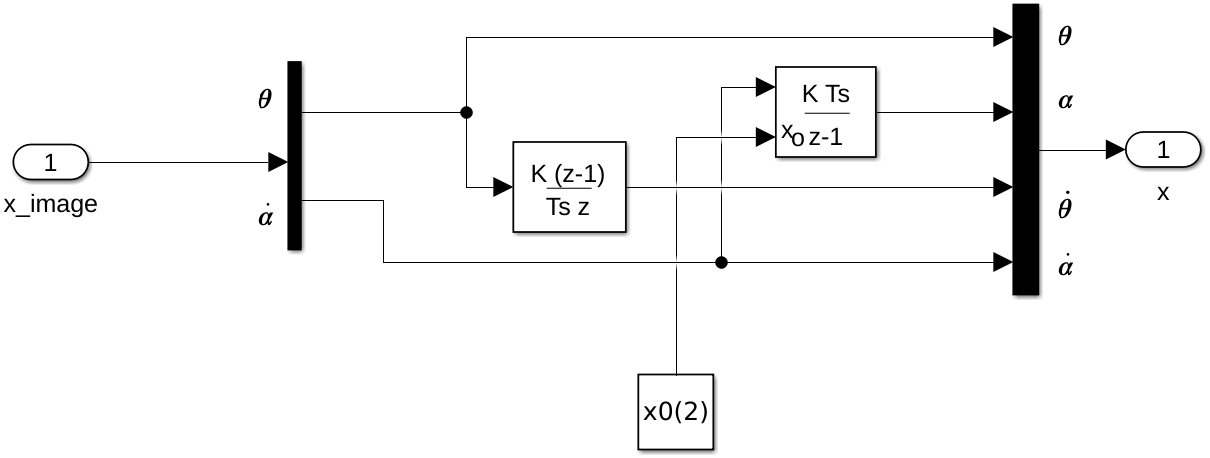
\includegraphics[width=12cm]{simulink_tp3_3_predicteur.png} 
		\caption{\textit{Schéma bloc du prédicteur avec signal discret}}
		\label{fig:simulink_tp3_3_predicteur}
\end{figure}
\vspace{0.5cm}

\quad Les cas d'études de la simulation sont encore les mêmes (table \ref{table:3}) mais on pense bien à fixer le pas de la simulation à $0.005$, sans quoi la discrétisation trop forte produit une simulation peu concluante. Les résultats sont représentés figure \ref{fig:robot_discret}. \\
Finalement, les courbes sont encore similaires aux deux parties précédentes 2.2 et 2.1, les oscillations sont seulement un peu plus amples. Donc, avec un bon intégrateur et une discrétisation qui a un pas suffisamment faible, on peut avoir un modèle très correct.

\begin{figure}[H]%
	\centering
	\noindent\makebox[\textwidth]{
		\subfloat[Cas 1]{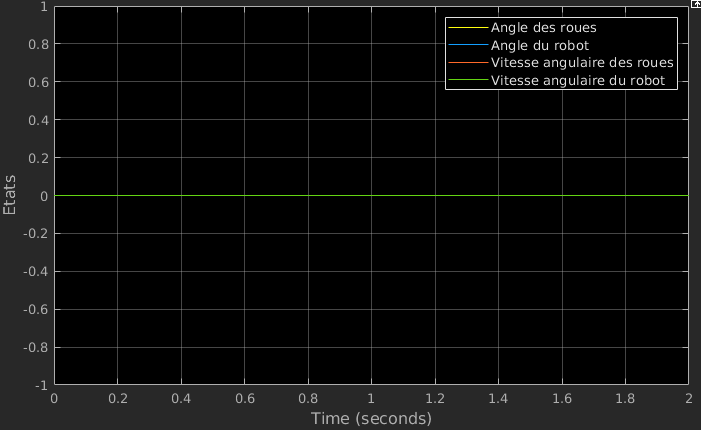
\includegraphics[width=9cm]{tp3_cas_31.png}} \qquad
		\subfloat[Cas 2]{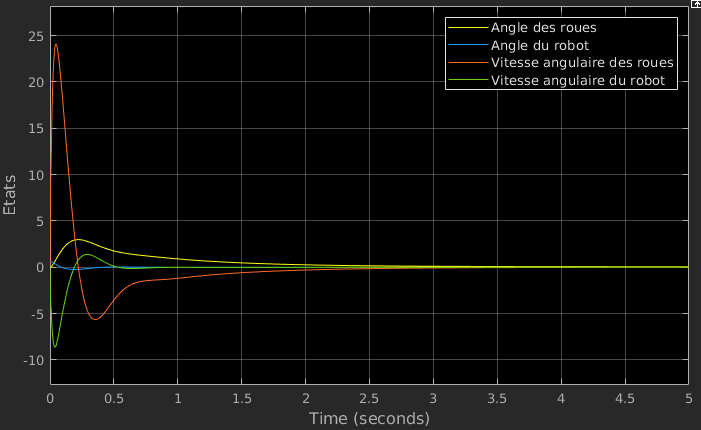
\includegraphics[width=9cm]{tp3_cas_32.png}}} \\
		\subfloat[Cas 3]{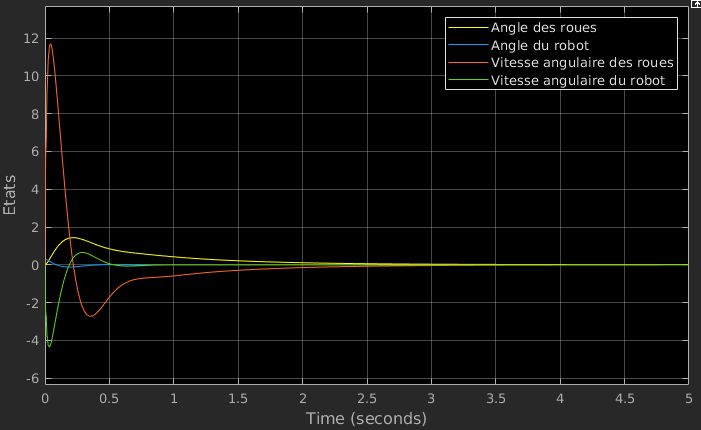
\includegraphics[width=9cm]{tp3_cas_33.png}}
		\captionsetup{justification=centering}
		\caption{\textit{Résultats du contrôle par retour de sortie du robot Lego pour différents états initiaux avec discrétisation}}
		\label{fig:robot_discret}%
\end{figure}
\vspace{0.5cm}


\newpage
\section{Robot Lego NXT}

\quad Au final, on a pu modéliser correctement le modèle du robot Lego NXT sur Simulink et vérifier qu'il fonctionne déjà dans ce cadre là. Maintenant, il n'y a plus qu'à l'implanter dans le logiciel qui sera utilisé dans le robot. On écrit ce logiciel en C. \\

\quad Plusieurs programmes sont déjà mis à notre disposition. Le logiciel se sépare en deux tâches, l'une va afficher les valeurs de $\alpha$, $\theta$ et de l'état $x$. La deuxième, celle qui nous intéresse, va permettre de maintenir la position verticale du robot. Elle se décompose en plusieurs modes. Le premier mode INIT\_MODE, initialise les variables du système. Le second mode CAL\_MODE, appelé après $4ms$, calibre le gyroscope à la verticale pendant $6s$ (il faut le tenir à la main). Enfin, le mode CONTROLE\_MODE calcul le contrôle et l'état du système toutes les $4ms$, c'est le coeur du fonctionnement du système. On remarque alors l'intérêt d'avoir simulé notre modèle avec discrétisation dans la partie 2.3 en prenant un pas de simulation de $5ms$. \\

\quad En séance de TP, nous avons écrit ce dernier mode. Il faut déjà écrire la fonction $estimateur$ qui calcul l'état du système $x=(\theta, \alpha, \dot\theta, \dot\alpha)$ à partir de l'état observé $y=(\theta_m, \dot\alpha)$ et du pas temporel (voir Listing \ref{listing:estimateur}). \\

\begin{lstlisting}[language=C, caption={Fonction estimateur}, label={listing:estimateur}]
void estimateur(float dt){
  float x_before = x[0];
  x[1] = x[1] + dt*y[1];
  x[3] = y[1];
  x[0] = y[0] + x[1];
  x[2] = (x[0]-x_before)/dt;
}
\end{lstlisting}

\quad Ensuite, nous avons écrit la fonction $controleur$ qui calcul la commande $u$ à appliquer au système en fonction de l'état courant du système (voir Listing \ref{listing:controleur}). \\

\begin{lstlisting}[language=C, caption={Fonction controleur}, label={listing:controleur}]
void controleur(){
  float somme = ue;
  float K[4] = {0.6700, 19.9055, 1.0747, 1.9614};
  for (int i=0; i<=3; i++){
    somme += K[i]*(x[i]-xe[i]);
  }
  u = somme;
}
\end{lstlisting}

\quad Puis, nous avons complété le mode CONTROLE\_MODE à l'aide de ces fonctions (voir Listing \ref{listing:controle_mode})

\begin{lstlisting}[language=C, caption={CONTROLE\_MODE}, label={listing:controle_mode}]
case(CONTROL_MODE):
  dt = delta_t();
  y[0] = getMotorAngle();
  y[1] = getGyro(gyro_offset);
  estimateur(dt);
  controleur();
  nxt_motors_set_command(u);
  break;
\end{lstlisting}

\quad Le logiciel est alors fini, il ne reste qu'à le compiler et le télécharger dans le robot Lego NXT.


\newpage
\section*{Conclusion}
\addcontentsline{toc}{section}{\protect\numberline{}Conclusion}

\quad Pour conclure ce projet, nous avons d'abord pu construire un modèle mathématique du système et le valider par simulation de plusieurs cas de figures avec différents paramètres. \\

\quad En premier, nous sommes passés par un système simple de pendule inversé qui modélise globalement le fonctionnement du robot. Cependant, pour se rapprocher de la réalité, nous avons introduit les vraies équations de la physique liées à la dynamique du robot en partie 2. Nous avons aussi choisi d'étudier des contrôles par retour d'état pour la théorie puis par retour de sortie avec des capteurs puisque le système réel fonctionne avec des capteurs. En effet, on a pas toujours accès à toutes les variables de sorties sur un système réel. Nous avons aussi choisi de simuler la discrétisation du système car l'implémentation du programme final utilise des variables discrètes.\\ 

\quad Finalement, au fur et à mesure on a pu valider nos modèles et obtenir des contrôles performants pour aboutir à un logiciel fonctionnel. 


\end{document}
